%
%   Chapter Datasets
%
%   Yong-Siang Shih
%   R.O.C.104.07
%
\chapter{Datasets}
\label{c:datasets}

In this chapter, we discuss the datasets used in this study, and
provide some statistics and analysis.

\section{Chinese Discourse Treebank (CDTB)}
\label{s:CDTB}
\subsection{Introduction}

Chinese Discourse Treebank (CDTB)~\citep{li2014building} is a discourse
corpus that contains 500 articles selected from the Chinese Treebank (CTB)~\citep{xue2005penn}.
Totally, it contains 2,342 paragraphs.
Inspired by RST and PDTB, they proposed the Connective-driven Dependency Tree (CDT)
scheme to annotate the documents.

In CDTB, each paragraph is represented as a discourse tree. The leaf nodes are the
elementary discourse units (EDUs) for the text, while internal nodes are discourse
relations between discourse units. This is very similar to RST-DT.

The set of discourse relation types is organized in a three-level hierarchy as
shown in Figure~\ref{i:three-level}.
The top-level categories have four relation types including causality, coordination,
transition, and explanation. The second level
have 17 types. The third level are the discourse connectives themselves.
As some connectives may be used for different relation types, there may
be multiple third-level connectives that have the same surface form under
different second-level relation types. For example, the connective
``并'' (and) appear in the following second-level relation types:
progressive, continue, explanation, and coordination.

% i:three-level
\begin{figure}[!htbp]
\begin{multicols}{2}
\begin{itemize}
  \item[] \textbf{causality}
  \begin{itemize}
    \item cause-result 
    \begin{itemize}
      \item[-] because \ldots
    \end{itemize}
    \item inference
    \begin{itemize}
      \item[-] so that \ldots
    \end{itemize}
    \item hypothetical
    \begin{itemize}
      \item[-] if \ldots
    \end{itemize}
    \item purpose
    \begin{itemize}
      \item[-] in order to \ldots
    \end{itemize}
    \item condition
    \begin{itemize}
      \item[-] only \ldots
    \end{itemize}
    \item background
    \begin{itemize}
      \item[-] background \ldots
    \end{itemize}
  \end{itemize}

  \item[] \textbf{transition}
  \begin{itemize}
    \item transition
    \begin{itemize}
      \item[-] but \ldots
    \end{itemize}
    \item concessive
    \begin{itemize}
      \item[-] although \ldots
    \end{itemize}
  \end{itemize}

  \vfill
  \columnbreak

  \item[] \textbf{coordination}
  \begin{itemize}
    \item coordination
    \begin{itemize}
      \item[-] and \ldots
    \end{itemize}
    \item continue
    \begin{itemize}
      \item[-] first \ldots second \ldots
    \end{itemize}
    \item progressive
    \begin{itemize}
      \item[-] in addition \ldots
    \end{itemize}
    \item selectional
    \begin{itemize}
      \item[-] or \ldots
    \end{itemize}
    \item inverse
    \begin{itemize}
      \item[-] compared with \ldots
    \end{itemize}
  \end{itemize}

  \item[] \textbf{explanation}
  \begin{itemize}
    \item explanation
    \begin{itemize}
      \item[-] which including \ldots
    \end{itemize}
    \item summary-elaboration
    \begin{itemize}
      \item[-] in a word \ldots
    \end{itemize}
    \item example
    \begin{itemize}
      \item[-] e.g. \ldots
    \end{itemize}
    \item evaluation
    \begin{itemize}
      \item[-] evaluation \ldots
    \end{itemize}
  \end{itemize}
\end{itemize}
\end{multicols}

\caption{\label{i:three-level} A three-level set of discourse relations in
CDTB. }
\end{figure}


For an explicit relation, once its second-level type is determined, the
third-level type is just its explicit connective. For an implicit relation,
a connective that could be inserted is annotated as its third-level type.
Sometimes there is no appropriate connective to be inserted. In such a case,
the relation is only annotated with a second-level relation type.

Consider the example sentences (S~\ref{sent:cdtb}) selected from CDTB. Its discourse
structure is shown in Figure~\ref{i:cdtb-tree}. The \textit{continue} relation between
discourse units (a-b) and (c) is implicit, but ``以后'' (later) can be inserted
as a connective as denoted by ``<以后>'' in (S~\ref{sent:cdtb}).
On the other hand, the explanation relation between (d) and (e-g)
does not have an inserted connective.


\begin{sent}{sent:cdtb}{}
    [\underline{尽管}浦东新区制定的法规性文件有些比较``粗'',]\textsuperscript{a}
    [有些\underline{还}只是暂行规定,]\textsuperscript{b}
    [有待<以后>在实践中逐步完善,]\textsuperscript{c}
    [\underline{但}这种法制紧跟经济和社会活动的做法,]\textsuperscript{d}
    [受到了国内外投资者的好评,]\textsuperscript{e}
    [他们认为,到浦东新区投资办事有章法,]\textsuperscript{f}
    [讲规矩,]\textsuperscript{g}
    [利益能得到保障。]\textsuperscript{h}

    (Although some regulatory documents for the Pudong New Area are "rough",
    and some regulations are still temporary and
    need to be refined gradually,
    the practice for regulations to closely follow economic and social activities
    are praised by domestic and foreign investors.
    Their view on investing in the Pudong New Area is that
    things are done methodologically,
    rules are followed,
    and their interest can be protected.)
\end{sent}

% i:cdtb-tree
\begin{figure}[!htbp]
\centering
\tikzset{every tree node/.style={align=center},
    level distance=40pt,
    sibling distance=6pt}
\begin{tikzpicture}
\Tree[.{concessive \\ 尽管 \ldots 但 (although \ldots but)}
       [.{continue \\ (以后) (later)}
         [.{coordination \\ 还 (still)}
           [ (a) ]
           [ (b) ]
         ]
         [ (c) ]
       ]
       [.{explanation}
         [ (d) ]
         [.{coordination}
           [ (e) ]
           [ (f) ]
           [ (g) ]
         ]
       ]
     ]

\end{tikzpicture}

\caption{\label{i:cdtb-tree} A discourse tree in CDTB. }
\end{figure}


Since we only consider explicit relations in this study, we will ignore
third-level relation types from now on to avoid confusion.
For an explicit relation, the second-level relation type and its explicit
connective can already uniquely determine its relation type.
When we refer to connective classes in the following section, we mean the
surface forms of connectives (i.e., instances of the same connective class
may have different relation types).

\subsection{Analysis}

During our experiments, we found some errors in the corpus including
duplicate annotations and erroneous positions, so we corrected
them. After the correction, there are 2,131 connective component instances
annotated for the explicit relations, and they form 1,813 connective instances.
The length distribution for the connectives are shown in Table~\ref{t:connective-length}.
The distribution is imbalance. Most connectives only have
one or two connective components. Also, while some connectives have many instances,
many connectives appear rarely. The frequencies for the connectives are shown
in Figure~\ref{i:freq}. There are totally 274 classes of connectives, but
147 of them appear only once.

% t:connective-length
\begin{table}[ht]
\centering
\begin{tabular}{|c|c|c|c|c|c|c|}
\hline
\bf \#Components        & 1    & 2   & 3  & 4 & 6 & 7 \\ \hline
\bf \#Connective Types  & 143  & 108 & 15 & 6 & 1 & 1 \\ \hline
\bf \#Instances         & 1544 & 235 & 24 & 8 & 1 & 1 \\ \hline
\end{tabular}
\caption{\label{t:connective-length} Lengths of connectives.}
This tables shows how many connective types have a specific length
and how many instances they totally appear. The number of types
is counted by the surface forms for the connectives.
\end{table}


% i:freq
\begin{figure}[!htbp]
\centering
    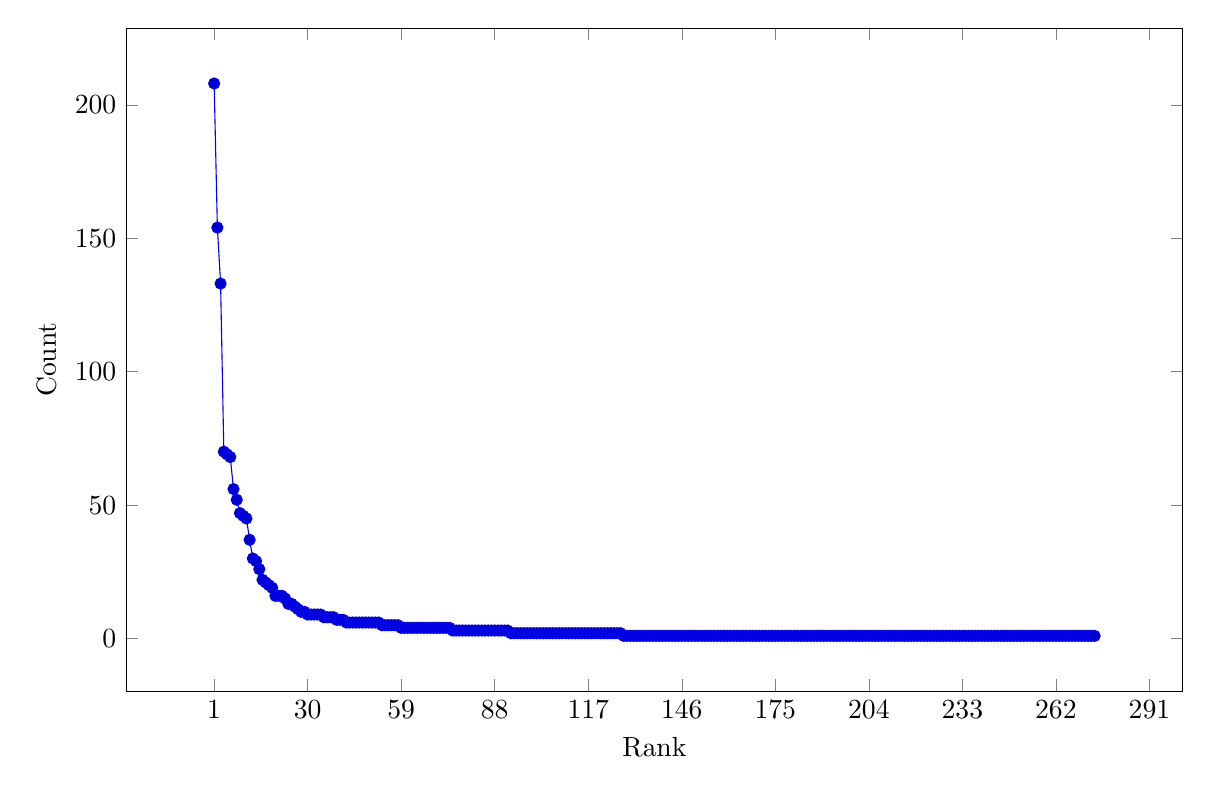
\begin{tikzpicture}
        \begin{axis}[
                width=15cm,
                height=10cm,
                xlabel=Rank,
                ylabel=Count,
                xtick={1,30,...,262,291},
                xticklabel style={/pgf/number format/assume math mode},
                yticklabel style={/pgf/number format/assume math mode},
            ]

            \addplot+[sharp plot] coordinates
            {
            (1,208)
            (2,154)
            (3,133)
            (4,70)
            (5,69)
            (6,68)
            (7,56)
            (8,52)
            (9,47)
            (10,46)
            (11,45)
            (12,37)
            (13,30)
            (14,29)
            (15,26)
            (16,22)
            (17,21)
            (18,20)
            (19,19)
            (20,16)
            (21,16)
            (22,16)
            (23,15)
            (24,13)
            (25,13)
            (26,12)
            (27,11)
            (28,10)
            (29,10)
            (30,9)
            (31,9)
            (32,9)
            (33,9)
            (34,9)
            (35,8)
            (36,8)
            (37,8)
            (38,8)
            (39,7)
            (40,7)
            (41,7)
            (42,6)
            (43,6)
            (44,6)
            (45,6)
            (46,6)
            (47,6)
            (48,6)
            (49,6)
            (50,6)
            (51,6)
            (52,6)
            (53,5)
            (54,5)
            (55,5)
            (56,5)
            (57,5)
            (58,5)
            (59,4)
            (60,4)
            (61,4)
            (62,4)
            (63,4)
            (64,4)
            (65,4)
            (66,4)
            (67,4)
            (68,4)
            (69,4)
            (70,4)
            (71,4)
            (72,4)
            (73,4)
            (74,4)
            (75,3)
            (76,3)
            (77,3)
            (78,3)
            (79,3)
            (80,3)
            (81,3)
            (82,3)
            (83,3)
            (84,3)
            (85,3)
            (86,3)
            (87,3)
            (88,3)
            (89,3)
            (90,3)
            (91,3)
            (92,3)
            (93,2)
            (94,2)
            (95,2)
            (96,2)
            (97,2)
            (98,2)
            (99,2)
            (100,2)
            (101,2)
            (102,2)
            (103,2)
            (104,2)
            (105,2)
            (106,2)
            (107,2)
            (108,2)
            (109,2)
            (110,2)
            (111,2)
            (112,2)
            (113,2)
            (114,2)
            (115,2)
            (116,2)
            (117,2)
            (118,2)
            (119,2)
            (120,2)
            (121,2)
            (122,2)
            (123,2)
            (124,2)
            (125,2)
            (126,2)
            (127,2)
            (128,1)
            (129,1)
            (130,1)
            (131,1)
            (132,1)
            (133,1)
            (134,1)
            (135,1)
            (136,1)
            (137,1)
            (138,1)
            (139,1)
            (140,1)
            (141,1)
            (142,1)
            (143,1)
            (144,1)
            (145,1)
            (146,1)
            (147,1)
            (148,1)
            (149,1)
            (150,1)
            (151,1)
            (152,1)
            (153,1)
            (154,1)
            (155,1)
            (156,1)
            (157,1)
            (158,1)
            (159,1)
            (160,1)
            (161,1)
            (162,1)
            (163,1)
            (164,1)
            (165,1)
            (166,1)
            (167,1)
            (168,1)
            (169,1)
            (170,1)
            (171,1)
            (172,1)
            (173,1)
            (174,1)
            (175,1)
            (176,1)
            (177,1)
            (178,1)
            (179,1)
            (180,1)
            (181,1)
            (182,1)
            (183,1)
            (184,1)
            (185,1)
            (186,1)
            (187,1)
            (188,1)
            (189,1)
            (190,1)
            (191,1)
            (192,1)
            (193,1)
            (194,1)
            (195,1)
            (196,1)
            (197,1)
            (198,1)
            (199,1)
            (200,1)
            (201,1)
            (202,1)
            (203,1)
            (204,1)
            (205,1)
            (206,1)
            (207,1)
            (208,1)
            (209,1)
            (210,1)
            (211,1)
            (212,1)
            (213,1)
            (214,1)
            (215,1)
            (216,1)
            (217,1)
            (218,1)
            (219,1)
            (220,1)
            (221,1)
            (222,1)
            (223,1)
            (224,1)
            (225,1)
            (226,1)
            (227,1)
            (228,1)
            (229,1)
            (230,1)
            (231,1)
            (232,1)
            (233,1)
            (234,1)
            (235,1)
            (236,1)
            (237,1)
            (238,1)
            (239,1)
            (240,1)
            (241,1)
            (242,1)
            (243,1)
            (244,1)
            (245,1)
            (246,1)
            (247,1)
            (248,1)
            (249,1)
            (250,1)
            (251,1)
            (252,1)
            (253,1)
            (254,1)
            (255,1)
            (256,1)
            (257,1)
            (258,1)
            (259,1)
            (260,1)
            (261,1)
            (262,1)
            (263,1)
            (264,1)
            (265,1)
            (266,1)
            (267,1)
            (268,1)
            (269,1)
            (270,1)
            (271,1)
            (272,1)
            (273,1)
            (274,1)
                };
        \end{axis}
    \end{tikzpicture}
\caption{\label{i:freq} Frequencies of connectives. }
\end{figure}



We list the top 25 classes of connectives in Figure~\ref{i:connective-types}.
Most of these connectives have only one component.

% i:connective-types
\begin{figure}[ht]
\centering
    \begin{tikzpicture}
        \begin{axis}[
            width=15cm,
            bar width = 7pt,
            enlarge x limits=0.05,
            symbolic x coords={
            并, 其中, 也, 而, 但, 还, 使, 以, 为, 同时,
            后, 由于, 因此, 如, 又, 为了, 因为, 而且, 如果, 後,
            此外, 虽然-但, 但是, 从而, 然而
            }, 
            ybar,
            nodes near coords,
            x tick label style={font=\small,align=center,rotate=70},
            xtick=data
          ]
            \addplot[ybar,fill=blue] coordinates {
                (并,  208)
                (其中,    154)
                (也,  133)
                (而,  70)
                (但,  69)
                (还,  68)
                (使,  56)
                (以,  52)
                (为,  47)
                (同时,    46)
                (后,  45)
                (由于,    37)
                (因此,    30)
                (如,  29)
                (又,  26)
                (为了,    22)
                (因为,    21)
                (而且,    20)
                (如果,    19)
                (後,  16)
                (此外,    16)
                (虽然-但, 16)
                (但是,    15)
                (从而,    13)
                (然而,    13)
            };
        \end{axis}
    \end{tikzpicture}
\caption{\label{i:connective-types} Top 25 Types. }
\end{figure}


While there are totally 274 classes of connectives, there are only 227 classes
of connective components found in the explicit relation annotations. This
is because many components can either be a single connective or link
with other components to form a parallel connective. We collect these
connectives and connective components to construct a connective lexicon
that has 274 entries and a component lexicon that has 227 entries.


Although many connectives appear rarely, there exist many spurious connective
candidates that do not actually have discourse meaning. This can be seen in
Figure~\ref{i:freq-detected}. We show the number of connective candidates
detected if we use string matching with the connective lexicon to extract
all connective candidates from the corpus. This problem is partly caused by the linking
ambiguities but the large number of spurious component candidates is a worse problem.
These spurious component candidates form a lot of spurious connective candidates.
In fact, if we could identify the correct
connective components, the total number of connective candidates they form
is only 2,249, and 1,813 of them are correct, which is about 80\% of these candidates.

% i:freq-detected
\begin{figure}[ht]
\centering
    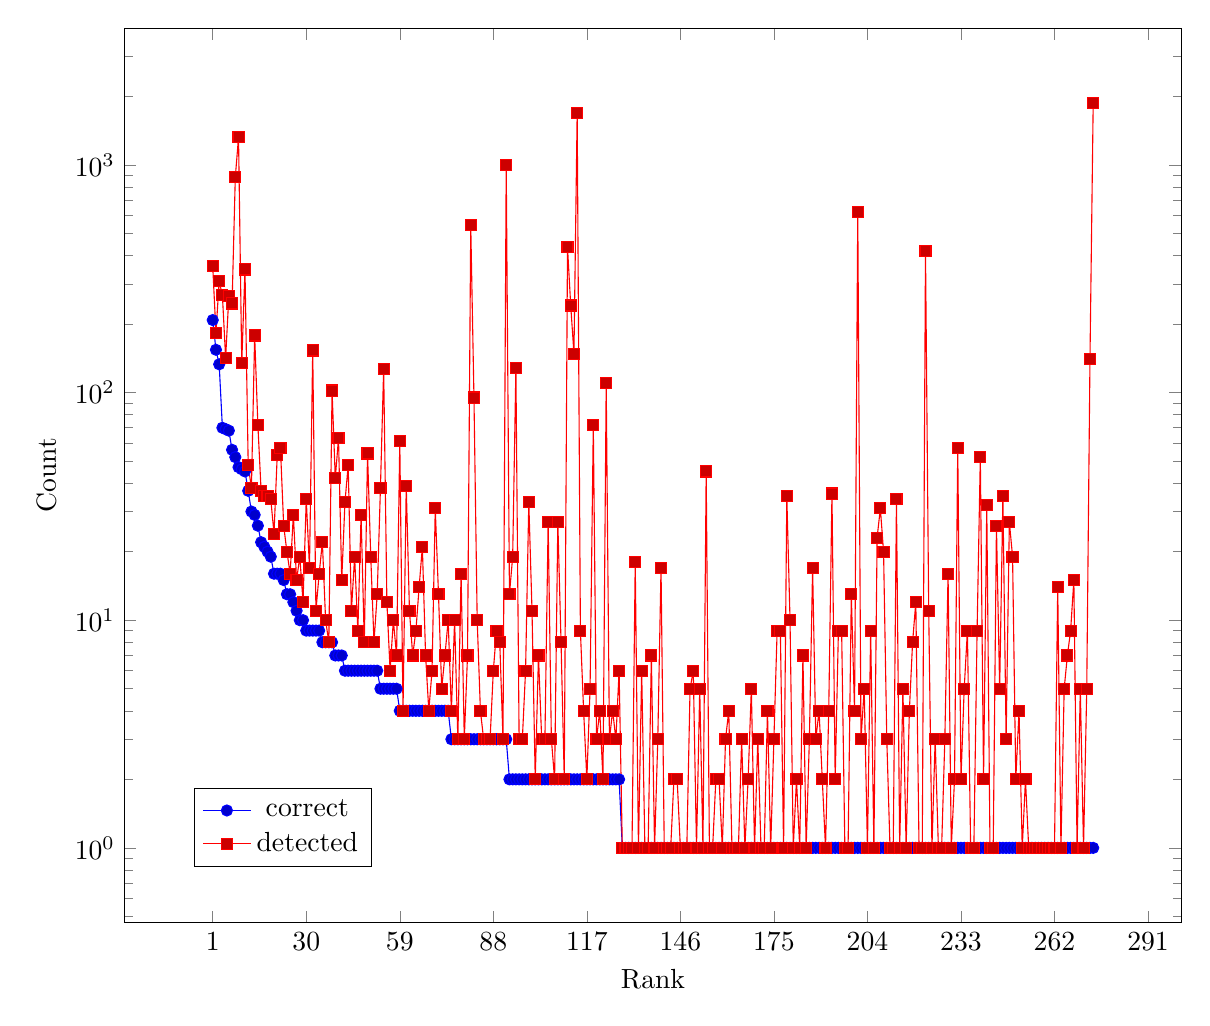
\begin{tikzpicture}
        \begin{axis}[
                width=15cm,
                xlabel=Rank,
                ylabel=Count,
                legend style={at={(0.15,0.15)},
                anchor=north},
                xtick={1,30,...,262,291},
                ymode=log,
            ]

            \addplot+[sharp plot] coordinates
            {
            (1,208)
            (2,154)
            (3,133)
            (4,70)
            (5,69)
            (6,68)
            (7,56)
            (8,52)
            (9,47)
            (10,46)
            (11,45)
            (12,37)
            (13,30)
            (14,29)
            (15,26)
            (16,22)
            (17,21)
            (18,20)
            (19,19)
            (20,16)
            (21,16)
            (22,16)
            (23,15)
            (24,13)
            (25,13)
            (26,12)
            (27,11)
            (28,10)
            (29,10)
            (30,9)
            (31,9)
            (32,9)
            (33,9)
            (34,9)
            (35,8)
            (36,8)
            (37,8)
            (38,8)
            (39,7)
            (40,7)
            (41,7)
            (42,6)
            (43,6)
            (44,6)
            (45,6)
            (46,6)
            (47,6)
            (48,6)
            (49,6)
            (50,6)
            (51,6)
            (52,6)
            (53,5)
            (54,5)
            (55,5)
            (56,5)
            (57,5)
            (58,5)
            (59,4)
            (60,4)
            (61,4)
            (62,4)
            (63,4)
            (64,4)
            (65,4)
            (66,4)
            (67,4)
            (68,4)
            (69,4)
            (70,4)
            (71,4)
            (72,4)
            (73,4)
            (74,4)
            (75,3)
            (76,3)
            (77,3)
            (78,3)
            (79,3)
            (80,3)
            (81,3)
            (82,3)
            (83,3)
            (84,3)
            (85,3)
            (86,3)
            (87,3)
            (88,3)
            (89,3)
            (90,3)
            (91,3)
            (92,3)
            (93,2)
            (94,2)
            (95,2)
            (96,2)
            (97,2)
            (98,2)
            (99,2)
            (100,2)
            (101,2)
            (102,2)
            (103,2)
            (104,2)
            (105,2)
            (106,2)
            (107,2)
            (108,2)
            (109,2)
            (110,2)
            (111,2)
            (112,2)
            (113,2)
            (114,2)
            (115,2)
            (116,2)
            (117,2)
            (118,2)
            (119,2)
            (120,2)
            (121,2)
            (122,2)
            (123,2)
            (124,2)
            (125,2)
            (126,2)
            (127,2)
            (128,1)
            (129,1)
            (130,1)
            (131,1)
            (132,1)
            (133,1)
            (134,1)
            (135,1)
            (136,1)
            (137,1)
            (138,1)
            (139,1)
            (140,1)
            (141,1)
            (142,1)
            (143,1)
            (144,1)
            (145,1)
            (146,1)
            (147,1)
            (148,1)
            (149,1)
            (150,1)
            (151,1)
            (152,1)
            (153,1)
            (154,1)
            (155,1)
            (156,1)
            (157,1)
            (158,1)
            (159,1)
            (160,1)
            (161,1)
            (162,1)
            (163,1)
            (164,1)
            (165,1)
            (166,1)
            (167,1)
            (168,1)
            (169,1)
            (170,1)
            (171,1)
            (172,1)
            (173,1)
            (174,1)
            (175,1)
            (176,1)
            (177,1)
            (178,1)
            (179,1)
            (180,1)
            (181,1)
            (182,1)
            (183,1)
            (184,1)
            (185,1)
            (186,1)
            (187,1)
            (188,1)
            (189,1)
            (190,1)
            (191,1)
            (192,1)
            (193,1)
            (194,1)
            (195,1)
            (196,1)
            (197,1)
            (198,1)
            (199,1)
            (200,1)
            (201,1)
            (202,1)
            (203,1)
            (204,1)
            (205,1)
            (206,1)
            (207,1)
            (208,1)
            (209,1)
            (210,1)
            (211,1)
            (212,1)
            (213,1)
            (214,1)
            (215,1)
            (216,1)
            (217,1)
            (218,1)
            (219,1)
            (220,1)
            (221,1)
            (222,1)
            (223,1)
            (224,1)
            (225,1)
            (226,1)
            (227,1)
            (228,1)
            (229,1)
            (230,1)
            (231,1)
            (232,1)
            (233,1)
            (234,1)
            (235,1)
            (236,1)
            (237,1)
            (238,1)
            (239,1)
            (240,1)
            (241,1)
            (242,1)
            (243,1)
            (244,1)
            (245,1)
            (246,1)
            (247,1)
            (248,1)
            (249,1)
            (250,1)
            (251,1)
            (252,1)
            (253,1)
            (254,1)
            (255,1)
            (256,1)
            (257,1)
            (258,1)
            (259,1)
            (260,1)
            (261,1)
            (262,1)
            (263,1)
            (264,1)
            (265,1)
            (266,1)
            (267,1)
            (268,1)
            (269,1)
            (270,1)
            (271,1)
            (272,1)
            (273,1)
            (274,1)
            };

            \addplot+[sharp plot] coordinates
            {
            (1,359)
            (2,183)
            (3,308)
            (4,267)
            (5,142)
            (6,265)
            (7,246)
            (8,883)
            (9,1321)
            (10,135)
            (11,347)
            (12,48)
            (13,38)
            (14,178)
            (15,72)
            (16,37)
            (17,35)
            (18,35)
            (19,34)
            (20,24)
            (21,53)
            (22,57)
            (23,26)
            (24,20)
            (25,16)
            (26,29)
            (27,15)
            (28,19)
            (29,12)
            (30,34)
            (31,17)
            (32,153)
            (33,11)
            (34,16)
            (35,22)
            (36,10)
            (37,8)
            (38,102)
            (39,42)
            (40,63)
            (41,15)
            (42,33)
            (43,48)
            (44,11)
            (45,19)
            (46,9)
            (47,29)
            (48,8)
            (49,54)
            (50,19)
            (51,8)
            (52,13)
            (53,38)
            (54,127)
            (55,12)
            (56,6)
            (57,10)
            (58,7)
            (59,61)
            (60,4)
            (61,39)
            (62,11)
            (63,7)
            (64,9)
            (65,14)
            (66,21)
            (67,7)
            (68,4)
            (69,6)
            (70,31)
            (71,13)
            (72,5)
            (73,7)
            (74,10)
            (75,4)
            (76,10)
            (77,3)
            (78,16)
            (79,3)
            (80,7)
            (81,545)
            (82,95)
            (83,10)
            (84,4)
            (85,3)
            (86,3)
            (87,3)
            (88,6)
            (89,9)
            (90,8)
            (91,3)
            (92,1000)
            (93,13)
            (94,19)
            (95,128)
            (96,3)
            (97,3)
            (98,6)
            (99,33)
            (100,11)
            (101,2)
            (102,7)
            (103,3)
            (104,3)
            (105,27)
            (106,3)
            (107,2)
            (108,27)
            (109,8)
            (110,2)
            (111,435)
            (112,241)
            (113,148)
            (114,1695)
            (115,9)
            (116,4)
            (117,2)
            (118,5)
            (119,72)
            (120,3)
            (121,4)
            (122,2)
            (123,110)
            (124,3)
            (125,4)
            (126,3)
            (127,6)
            (128,1)
            (129,1)
            (130,1)
            (131,1)
            (132,18)
            (133,1)
            (134,6)
            (135,1)
            (136,1)
            (137,7)
            (138,1)
            (139,3)
            (140,17)
            (141,1)
            (142,1)
            (143,1)
            (144,2)
            (145,2)
            (146,1)
            (147,1)
            (148,1)
            (149,5)
            (150,6)
            (151,1)
            (152,5)
            (153,1)
            (154,45)
            (155,1)
            (156,1)
            (157,2)
            (158,2)
            (159,1)
            (160,3)
            (161,4)
            (162,1)
            (163,1)
            (164,1)
            (165,3)
            (166,1)
            (167,2)
            (168,5)
            (169,1)
            (170,3)
            (171,1)
            (172,1)
            (173,4)
            (174,1)
            (175,3)
            (176,9)
            (177,9)
            (178,1)
            (179,35)
            (180,10)
            (181,1)
            (182,2)
            (183,1)
            (184,7)
            (185,1)
            (186,3)
            (187,17)
            (188,3)
            (189,4)
            (190,2)
            (191,1)
            (192,4)
            (193,36)
            (194,2)
            (195,9)
            (196,9)
            (197,1)
            (198,1)
            (199,13)
            (200,4)
            (201,622)
            (202,3)
            (203,5)
            (204,1)
            (205,9)
            (206,1)
            (207,23)
            (208,31)
            (209,20)
            (210,3)
            (211,1)
            (212,1)
            (213,34)
            (214,1)
            (215,5)
            (216,1)
            (217,4)
            (218,8)
            (219,12)
            (220,1)
            (221,1)
            (222,419)
            (223,11)
            (224,1)
            (225,3)
            (226,1)
            (227,1)
            (228,3)
            (229,16)
            (230,1)
            (231,2)
            (232,57)
            (233,2)
            (234,5)
            (235,9)
            (236,1)
            (237,1)
            (238,9)
            (239,52)
            (240,2)
            (241,32)
            (242,1)
            (243,1)
            (244,26)
            (245,5)
            (246,35)
            (247,3)
            (248,27)
            (249,19)
            (250,2)
            (251,4)
            (252,1)
            (253,2)
            (254,1)
            (255,1)
            (256,1)
            (257,1)
            (258,1)
            (259,1)
            (260,1)
            (261,1)
            (262,1)
            (263,14)
            (264,1)
            (265,5)
            (266,7)
            (267,9)
            (268,15)
            (269,1)
            (270,5)
            (271,1)
            (272,5)
            (273,140)
            (274,1873)
            };

            %\addplot+[sharp plot] coordinates
            %{
            %(1,212)
            %(2,154)
            %(3,182)
            %(4,85)
            %(5,110)
            %(6,106)
            %(7,57)
            %(8,53)
            %(9,47)
            %(10,61)
            %(11,49)
            %(12,41)
            %(13,36)
            %(14,30)
            %(15,39)
            %(16,24)
            %(17,24)
            %(18,31)
            %(19,31)
            %(20,18)
            %(21,27)
            %(22,18)
            %(23,22)
            %(24,18)
            %(25,13)
            %(26,13)
            %(27,13)
            %(28,10)
            %(29,10)
            %(30,9)
            %(31,16)
            %(32,12)
            %(33,9)
            %(34,9)
            %(35,8)
            %(36,8)
            %(37,8)
            %(38,8)
            %(39,9)
            %(40,7)
            %(41,8)
            %(42,7)
            %(43,13)
            %(44,6)
            %(45,6)
            %(46,6)
            %(47,10)
            %(48,6)
            %(49,6)
            %(50,11)
            %(51,6)
            %(52,8)
            %(53,5)
            %(54,8)
            %(55,5)
            %(56,6)
            %(57,6)
            %(58,6)
            %(59,13)
            %(60,4)
            %(61,4)
            %(62,5)
            %(63,5)
            %(64,6)
            %(65,4)
            %(66,5)
            %(67,5)
            %(68,4)
            %(69,4)
            %(70,16)
            %(71,6)
            %(72,4)
            %(73,6)
            %(74,6)
            %(75,3)
            %(76,5)
            %(77,3)
            %(78,5)
            %(79,3)
            %(80,4)
            %(81,5)
            %(82,8)
            %(83,4)
            %(84,4)
            %(85,3)
            %(86,3)
            %(87,3)
            %(88,6)
            %(89,4)
            %(90,4)
            %(91,3)
            %(92,4)
            %(93,3)
            %(94,5)
            %(95,2)
            %(96,2)
            %(97,2)
            %(98,6)
            %(99,2)
            %(100,2)
            %(101,2)
            %(102,2)
            %(103,2)
            %(104,2)
            %(105,3)
            %(106,3)
            %(107,2)
            %(108,3)
            %(109,2)
            %(110,2)
            %(111,2)
            %(112,2)
            %(113,2)
            %(114,2)
            %(115,2)
            %(116,2)
            %(117,2)
            %(118,2)
            %(119,3)
            %(120,2)
            %(121,2)
            %(122,2)
            %(123,6)
            %(124,2)
            %(125,2)
            %(126,2)
            %(127,4)
            %(128,1)
            %(129,1)
            %(130,1)
            %(131,1)
            %(132,3)
            %(133,1)
            %(134,4)
            %(135,1)
            %(136,1)
            %(137,6)
            %(138,1)
            %(139,1)
            %(140,3)
            %(141,1)
            %(142,1)
            %(143,1)
            %(144,1)
            %(145,1)
            %(146,1)
            %(147,1)
            %(148,1)
            %(149,1)
            %(150,1)
            %(151,1)
            %(152,1)
            %(153,1)
            %(154,1)
            %(155,1)
            %(156,1)
            %(157,2)
            %(158,1)
            %(159,1)
            %(160,1)
            %(161,1)
            %(162,1)
            %(163,1)
            %(164,1)
            %(165,3)
            %(166,1)
            %(167,1)
            %(168,2)
            %(169,1)
            %(170,1)
            %(171,1)
            %(172,1)
            %(173,1)
            %(174,1)
            %(175,1)
            %(176,1)
            %(177,1)
            %(178,1)
            %(179,1)
            %(180,1)
            %(181,1)
            %(182,1)
            %(183,1)
            %(184,1)
            %(185,1)
            %(186,2)
            %(187,3)
            %(188,1)
            %(189,1)
            %(190,1)
            %(191,1)
            %(192,2)
            %(193,1)
            %(194,1)
            %(195,2)
            %(196,1)
            %(197,1)
            %(198,1)
            %(199,13)
            %(200,1)
            %(201,1)
            %(202,1)
            %(203,1)
            %(204,1)
            %(205,1)
            %(206,1)
            %(207,1)
            %(208,1)
            %(209,2)
            %(210,3)
            %(211,1)
            %(212,1)
            %(213,1)
            %(214,1)
            %(215,1)
            %(216,1)
            %(217,1)
            %(218,2)
            %(219,1)
            %(220,1)
            %(221,1)
            %(222,1)
            %(223,6)
            %(224,1)
            %(225,2)
            %(226,1)
            %(227,1)
            %(228,1)
            %(229,1)
            %(230,1)
            %(231,1)
            %(232,1)
            %(233,2)
            %(234,1)
            %(235,1)
            %(236,1)
            %(237,1)
            %(238,1)
            %(239,1)
            %(240,1)
            %(241,2)
            %(242,1)
            %(243,1)
            %(244,2)
            %(245,1)
            %(246,3)
            %(247,1)
            %(248,14)
            %(249,1)
            %(250,1)
            %(251,1)
            %(252,1)
            %(253,1)
            %(254,1)
            %(255,1)
            %(256,1)
            %(257,1)
            %(258,1)
            %(259,1)
            %(260,1)
            %(261,1)
            %(262,1)
            %(263,1)
            %(264,1)
            %(265,2)
            %(266,3)
            %(267,4)
            %(268,5)
            %(269,1)
            %(270,3)
            %(271,1)
            %(272,1)
            %(273,1)
            %(274,5)
            %};
            %\legend{correct,detected,detected for correct components}
            \legend{correct,detected}
        \end{axis}
    \end{tikzpicture}
\caption{\label{i:freq-detected} Frequencies of annotated connectives vs. detected connectives. }
\end{figure}


The problem caused by spurious component candidates is best illustrated in
Figure~\ref{i:linking-ambig-chart}. When correct components are identified,
the connective candidates formed by these components are limited.
Most of the components involve in only one connective, meaning that the correct linking
is known. The greatest linking ambiguity is only 5. However, when there are
spurious components, there exist a component candidate that involves in as many
as 240 connective candidates.

% i:linking-ambig-chart
\begin{figure}[ht]
\centering
    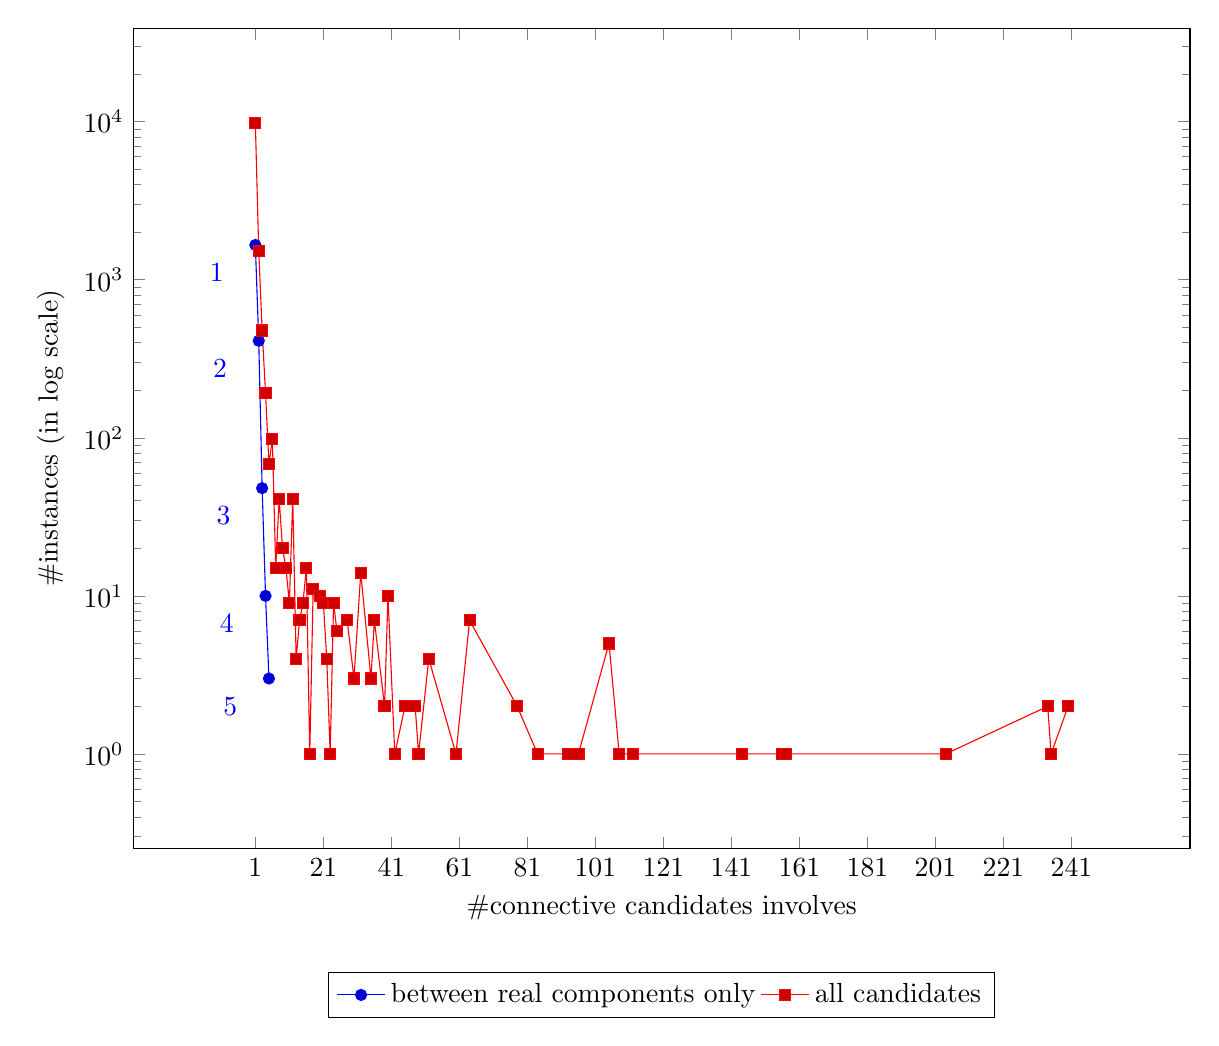
\begin{tikzpicture}
        \begin{axis}[
            width=15cm,
            height=12cm,
            enlargelimits=0.15,
            legend style={at={(0.5,-0.15)},
              anchor=north,legend columns=-1},
            xtick={1,21,...,245},
            xlabel={\#connective candidates involves},
            ylabel={\#instances (in log scale)},
            ymode=log,
            ]
        \addplot+[
                nodes near coords,
                every node near coord/.append style={xshift=-20, yshift=-10},
                nodes near coords align={horizontal},
                point meta=x,
                ] coordinates {
        (1,1659)
        (2,411)
        (3,48)
        (4,10)
        (5,3)
        };
        \addplot coordinates {
        (1,9827)
        (2,1525)
        (3,477)
        (4,191)
        (5,68)
        (6,98)
        (7,15)
        (8,41)
        (9,20)
        (10,15)
        (11,9)
        (12,41)
        (13,4)
        (14,7)
        (15,9)
        (16,15)
        (17,1)
        (18,11)
        (20,10)
        (21,9)
        (22,4)
        (23,1)
        (24,9)
        (25,6)
        (28,7)
        (30,3)
        (32,14)
        (35,3)
        (36,7)
        (39,2)
        (40,10)
        (42,1)
        (45,2)
        (48,2)
        (49,1)
        (52,4)
        (60,1)
        (64,7)
        (78,2)
        (84,1)
        (93,1)
        (96,1)
        (105,5)
        (108,1)
        (112,1)
        (144,1)
        (156,1)
        (157,1)
        (204,1)
        (234,2)
        (235,1)
        (240,2)
        };
        \legend{between real components only,all candidates}
        \end{axis}
    \end{tikzpicture}
\caption{\label{i:linking-ambig-chart} Number of connective candidates a component candidate involes. }
\end{figure}


For relation type ambiguity, we list the number of relation types a
connective used for explicit relations in the corpus in Table~\ref{t:connective-type}.
While most connective classes are only used for 1 relation type,
the ambiguous connectives have many instances.

% t:connective-type
\begin{table}[ht]
\centering
\begin{tabular}{|c|c|c|c|c|c|}
\hline
\#Top-level Relation Types & 1    & 2   & 3   & 4   & 5  \\ \hline
\#Connective Classes       & 258  & 15  & 1   & -   & -  \\ \hline
\#Instances                & 1388 & 355 & 70  & -   & -  \\

\hhline{|=|=|=|=|=|=|}

\#2nd-level Relation Types & 1    & 2   & 3   & 4   & 5  \\ \hline
\#Connective Classes       & 243  & 24  & 5   & 1   & 1  \\ \hline
\#Instances                & 1030 & 379 & 126 & 208 & 70 \\ \hline

\end{tabular}
\caption{\label{t:connective-type} Relation ambiguity of connectives. }
\end{table}


Table~\ref{t:argument-num} shows the number of arguments for the 1,813 explicit
relations. Most relations only have two arguments, but there are relations
that have as many as 7 arguments. The number of arguments does not always
match with the number of connective components in each relation. The same
connective can also have different number of arguments when used in
different relations. Single connectives can have as many as 6 arguments
as shown in (S~\ref{sent:same-time}), and in (S~\ref{sent:medal}),
the connective 除-外-还 (in addition to \ldots also)
has three components, but it only have two arguments.

% t:argument-num
\begin{table}[ht]
\centering
\begin{tabular}{|c|c|c|c|c|c|c|}
\hline

\#Arguments              & 2    & 3   & 4   & 5   & 6  & 7  \\ \hline
\#Instances              & 1688 & 85  & 33  & 4   & 2  & 1  \\ \hline

\end{tabular}
\caption{\label{t:argument-num} Number of arguments for each explicit relation. }
\end{table}


\begin{sent}{sent:same-time}{}
    [允许中资企业保留一定限额外汇收入,可以促使企业加强经济核算,]
    [降低生产经营成本,]
    [减少企业买卖外汇的支出,]
    [\underline{同时}可消除中外资企业在结汇方面的差别待遇,]
    [完善外汇市场运作和人民币汇率形成机制,]
    [扩大金融机构外汇存贷款业务。]
    (Allowing Chinese companies to retain a certain quota of foreign exchange earnings
     may encourage enterprises to enhance economic accounting.
     This reduces production and operation costs, and the expenses for foreign
     exchanges.  At the same time, it eliminates the different treatments between
     Chinese and foreign-funded enterprises in terms of foreign exchange settlement,
     improving the operation of the foreign exchange market and the RMB
     exchange rate formation mechanism, expanding the foreign currency deposits and
     loans of financial institutions.)
\end{sent}

\begin{sent}{sent:medal}{}
    [\underline{除}戈杰安夺得金牌\underline{外},]
    [米洛索维奇\underline{还}摘取铜牌。]
    (In addition to Gogean's gold medal, Milosovici also won the bronze medal.)
\end{sent}

\section{NTU PN-Gram Corpus}
\label{s:pn-corpus}

NTU PN-Gram Corpus~\citep{yu2012development} is a large-scale corpus that was
constructed by POS-tagging the Chinese texts selected from the ClueWeb09
dataset~\citep{callan2009clueweb09}. In NTU PN-Gram, there are totally 173,741,587
web pages containing 141,179,769,123 tokens.

Recently, efficient methods to estimate word embeddings have been developed.
These methods learn the distributed representation for each word that encodes
syntactic and semantic patterns in a fixed-dimensional vector.
These vectors exhibit interesting properties. For example,
\cite{mikolov2013linguistic} pointed out that there exist linear regularities
between these vectors:

$$ vector('king') - vector('man') + vector('woman') \approx vector('queen') $$

Therefore, we investigate whether these vectors are useful for solving
discourse issues. Due to the limitation of computation powers, we use
a subset of NTU PN-Gram that was extracted by \cite{huang2014interpretation}
to train our word embeddings. These sentences were extracted on the basis of the following three conditions:

\begin{enumerate}
\item Each sentence must have exactly two clauses.
\item Each sentence must have exactly one instance of connective.
\item Each of the two clauses must not have more than 20 Chinese characters.
\end{enumerate}

We use an intermediate result that contains 43,010,050 sentences and eliminate
the duplicate sentences. The result are 21,217,147 sentences, containing
326,996,602 tokens. These sentences are used to train word embeddings.
We have created 400-dimensional embeddings by GloVe tool~\citep{pennington2014glove}
and word2vec tool~\citep{mikolov2013efficient,mikolov2013distributed} with
continuous skip-gram model and continuous bag-of-words model.
These vectors are used as features as discussed in Chapter~\ref{c:method}.


\section{Linking Directions of Connective Components}

Discourse connectives serve as linking elements that connect discourse units.
There are three kinds of linking directions~\citep{li1989mandarin}:
(1) forward-linking elements that are linked with the next discourse unit,
(2) backward-linking elements that are linked with the previous discourse unit,
and (3) couple-linking elements that exist in two discourse units~\citep{chen1994contextual}.
Such linking directions could be useful for identifying the positions of arguments
for a given connective.

We selected 301 connective components annotated with their possible
linking directions from the 808 discourse connectives collected by
\cite{huang2014interpretation}. The linking directions are used as features
for our argument extraction.
